\documentclass[a4paper]{article}

%% Language and font encodings
\usepackage[english]{babel}
\usepackage[utf8x]{inputenc}
\usepackage[T1]{fontenc}

%% Sets page size and margins
\usepackage[a4paper,top=3cm,bottom=2cm,left=3cm,right=3cm,marginparwidth=1.75cm]{geometry}

%% Useful packages
\usepackage{amsmath}
\usepackage{amsfonts}
\usepackage{graphicx}
\usepackage[colorinlistoftodos]{todonotes}
\usepackage[colorlinks=true, allcolors=blue]{hyperref}
\usepackage{subfig}
\usepackage{xcolor}

\newcommand{\aw}[1]{{\color{blue} [AW: #1]}}
\newcommand{\jm}[1]{{\color{red} [JM: #1]}}
\newcommand{\ap}[1]{{\color{red} [AP: #1]}}

\title{Non-Periodic Edge States \footnote{ \aw{I prefer ``Edge States in Disordered Media''. The edge states may be periodic; the point is that we are studying such states in a medium (material) which is not. The term ``disordered'' is appropriate: it is not just that the pattern of the medium doesn't repeat itself, the material actually has no order: seeing what the material looks like in one place doesn't tell you very much about what it looks like in another because the atomic positions and onsite potentials are random. In, for example, a ``quasi-crystal'' the structure of the medium is ordered in the sense that it can be generated by a deterministic algorithm. This is not true for the media we are considering.} } }
\author{Jonathan Michala and Alexander Pierson}

\begin{document}

\aw{some things I want to make a note of:} 
\begin{itemize}
\item We have to make the bibliography: I can show you how to do this (it's a pain) using BibDesk
\end{itemize}

\newpage

\maketitle

\section{Background}
\aw{This you should be able to mostly lift from the Summer project. The main points are (1) controlling wave propagation is of significant interest for a range of applications: acoustics, electromagnetics, quantum mechanics... (2) particular interest in ways of controlling waves which are robust against imperfections in the medium/device (3) in ``topological insulators'' it is observed that waves which propagate at the edge of such media (edge states) are highly robust against perturbations, related with topological invariants associated with the bulk Hamiltonian (Chern number) (4) The aim of this project is to investigate to what extent this story (topological invariants and robust edge states) generalizes when the medium is strongly disordered i.e. we make a perturbation such that the medium is no longer periodic at all because of onsite potentials which vary significantly across the material and varying atomic positions. Good to contrast with the summer when we considered robustness of edge states to strong perturbations on the edge. Here we are studying perturbations of the \emph{whole medium}. Note also that we are considering a case where the usual topological invariant doesn't seem to be relevant at all since the medium is not periodic. This is where the Loring index comes in: it is an index which agrees with the Chern number when the medium is periodic, but since it is not defined through Bloch states it is well defined when the medium is not periodic (aperiodic) as well.}
\section{Loring Index} \aw{Note on title: let's call it the Bott index as in 2009HastingsLoring} \\

\aw{I would start with e.g. ``We start by introducing the Bott index abstractly, we discuss its relevance in physics below. (new paragraph) It is well known that a set of $n$ Hermitian matrices which commute may be simultaneously diagonalized, i.e.... Given a set of $n$ Hermitian matrices which \emph{almost} commute, i.e....''} \\

\aw{We can then talk about physics below ``The Bott index can be used to define a local topological index in a disordered medium as follows...'' } \\

\aw{Another thing (I apologize for being a little loose when I have talked about this in our meetings): our audience for this report is mathematicians. So let's not talk about ``eigenstates'' until we are talking about physics. At that point we should mention ``it is common in quantum mechanics to refer to eigenvectors of self-adjoint operators as eigenstates''} \\

Let $\Psi$ be a state in two dimensions with entries $\Psi_{m,n}$, where $m$ describes location with respect to one dimension (whether that be an $x$-coordinate in $\mathbb{R}^2$ or a cell index along an edge) and where $n$ describes location with respect to the other dimension.
Define $X$ and $Y$ to be an operators that act on a state $\Psi$ in the following way:
$$(X \Psi)_{m,n} = m\Psi_{m,n}, \quad (Y \Psi)_{m,n} = n\Psi_{m,n}.$$
Eigenstates of these operators are localized in their corresponding dimensions.
Therefore, when looking for localized eigenstates of a system whose Hamiltonian is $H$, our aim is to find simultaneous eigenstates of all three operators $H$, $X$, and $Y$.\\
This is not always possible, however.
Suppose $A_1,...,A_n$ are Hermitian matrices that all commute with each other.
Then, they can be simultaneously diagonalized, i.e. $U^\star A_i U$ is diagonal for all $i \in \{1,...,n\}$ for some unitary matrix $U$.
So if $H$, $X$, and $Y$ commute, we can find simultaneous eigenstates of them.
Now, suppose $A_1,...,A_n$ do not all commute, but their commutators are bounded:
$$[A_i,A_j] \leq \delta \quad \forall\; i,j \in \{1,...,n\}$$
for some $\delta$.
If $n = 2$, there must exist some $\widetilde{A}_1, \widetilde{A}_2$ such that they commute and satisfy:
$$||\widetilde{A}_1 - A_1||, ||\widetilde{A}_2 - A_2|| \leq \epsilon(\delta)$$
where $\epsilon(\delta) \ll \delta$ \jm{Is this correct?} \aw{I think better to just say $\epsilon(\delta) \rightarrow 0$ as $\delta \rightarrow 0$} and where $||M||$ denotes the largest eigenvalue of $M$.\\
But if $n = 3$, there may or may not exist $\widetilde{A}_1, \widetilde{A}_2, \widetilde{A}_3$ such that they all commute with each other and satisfy:
$$||\widetilde{A}_i - A_i|| \leq \epsilon(\delta), \quad \i \in \{1,2,3\}.$$
This existence holds if and only if
$$\frac{1}{2}\; \text{sig} \begin{pmatrix}
A_3 & A_1 + iA_2\\
A_1 - iA_2 & - A_3
\end{pmatrix} = 0$$
where sig$(M)$ is the signature, or number of positive eigenvalues minus negative eigenvalues, of $M$. This is known as the Bott Index of three matrices.
 of all three of these matrices, i.e. finding $v$ such that $(X - \lambda_1)v = 0$, $(Y - \lambda_2)v = 0$, and $(H-\lambda_3)v = 0$, for real $\lambda_1,\lambda_2,\lambda_3$. This is equivalent(Annals of Physics ref) to finding near-zero eigenvalues of the matrix
$$B(X - \lambda_1, Y - \lambda_2, H - \lambda_3) =
\begin{pmatrix}
H - \lambda_3 & (X - \lambda_1) + i(Y - \lambda_2)\\
(X - \lambda_1) - i(Y - \lambda_2) & - (H - \lambda_3)
\end{pmatrix}.$$
Thus, if this matrix has an eigenvalue less than a specified norm $\epsilon$, we say that \aw{it is $(\lambda_1,\lambda_2,\lambda_3)$ that is in the joint pseudo-spectrum: the pseudo-spectrum is a generalization of the spectrum (the set of eigenvalues), and the joint pseudo-spectrum is a generalization of the joint spectrum} is in the joint pseudo-spectrum of the given lattice. We can also compute the Loring index of $(\lambda_1,\lambda_2,\lambda_3)$ triples which is defined as the signature of $B$. \aw{This is a good start - you have clearly identified what the index measures. See my comments above, though.} \\\\
To compute the signature of $B$ efficiently, we use the $LDL^T$ decomposition of $B$. $D$ is a block diagonal matrix with blocks of either size $1 \times 1$ or $2 \times 2$. Let $a$ and $b$ be the number of positive and negative $1 \times 1$ blocks in $D$, respectively. By J.R. Bunch, L. Kaufman (Need ref), the signature of $B$ is equivalent to the signature of $D$ which is $a - b$. \aw{we should identify why $L D L^T$ works, e.g. ``it is known (see ref...) that the signature of $B$ equals the signature of the diagaonal matrix $D$ which appears in $L D L^T$ factorization''}

\section{Loring Index in Haldane Model}

\aw{Good idea to have this section. We should motivate what we do here, e.g. ``We now show numerically that the Bott index is equal to the Chern number where both are defined (i.e. when the medium is periodic so that the eigenstates of the Hamiltonian are Bloch states)'' }	\\

\aw{We should mention the issue with boundary conditions and having to shift the $X$ and $Y$ operators}

In the Haldane Model, $m$ and $n$ are the indices of cells on a hexagonal, atomic lattice, where each cell has two sites, labeled $A$ and $B$.
Thus we define our $X$ and $Y$ operators as follows:
$$X_{i,i} = \left\lfloor \frac{i-1}{2} \right\rfloor \;\text{mod}\;m, \quad\quad Y_{i,i} = \left\lfloor \frac{i-1}{2m} \right\rfloor$$
with $X_{i,j} = Y_{i,j} = 0$ for $i \neq j$. 
We compute the pseudo-spectrum and Loring index on the Haldane model lattice with complex hopping and see that in the topological case, the Loring index behave much like the Chern number: on a lattice with edges, the index is $+1$ on the interior and transitions to 0 across the edge; on a periodic lattice, the index is $+1$ everywhere. In the trivial case we see a Loring index of 0 everywhere on edged and periodic lattices, which is analogous to the Chern number. This is shown in Figure \ref{fig:Loring Haldane}.
\begin{figure}
\centering
\subfloat{{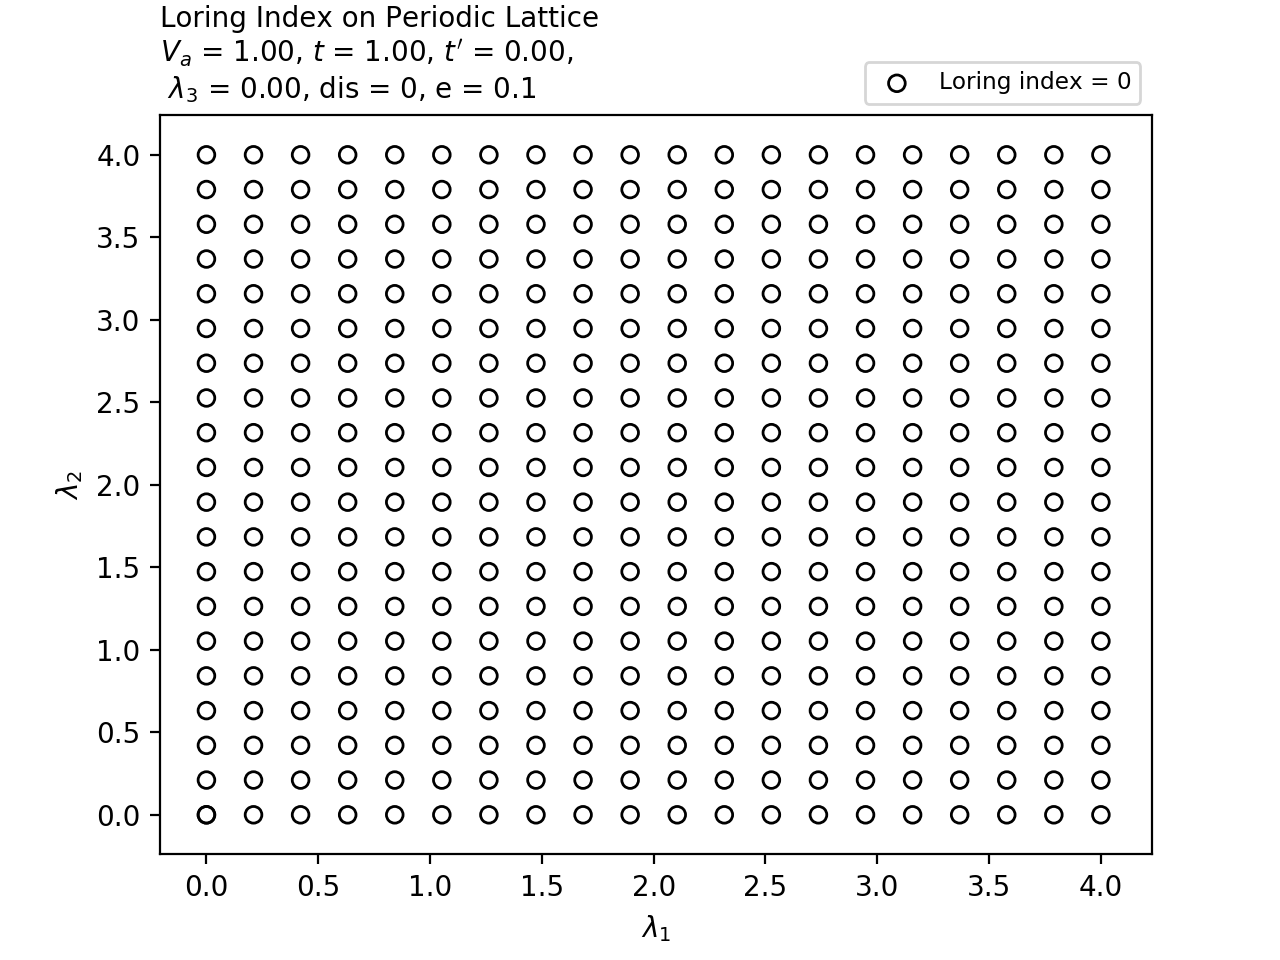
\includegraphics[width=.45\linewidth]{figures/periodic_triv} }}%
\subfloat{{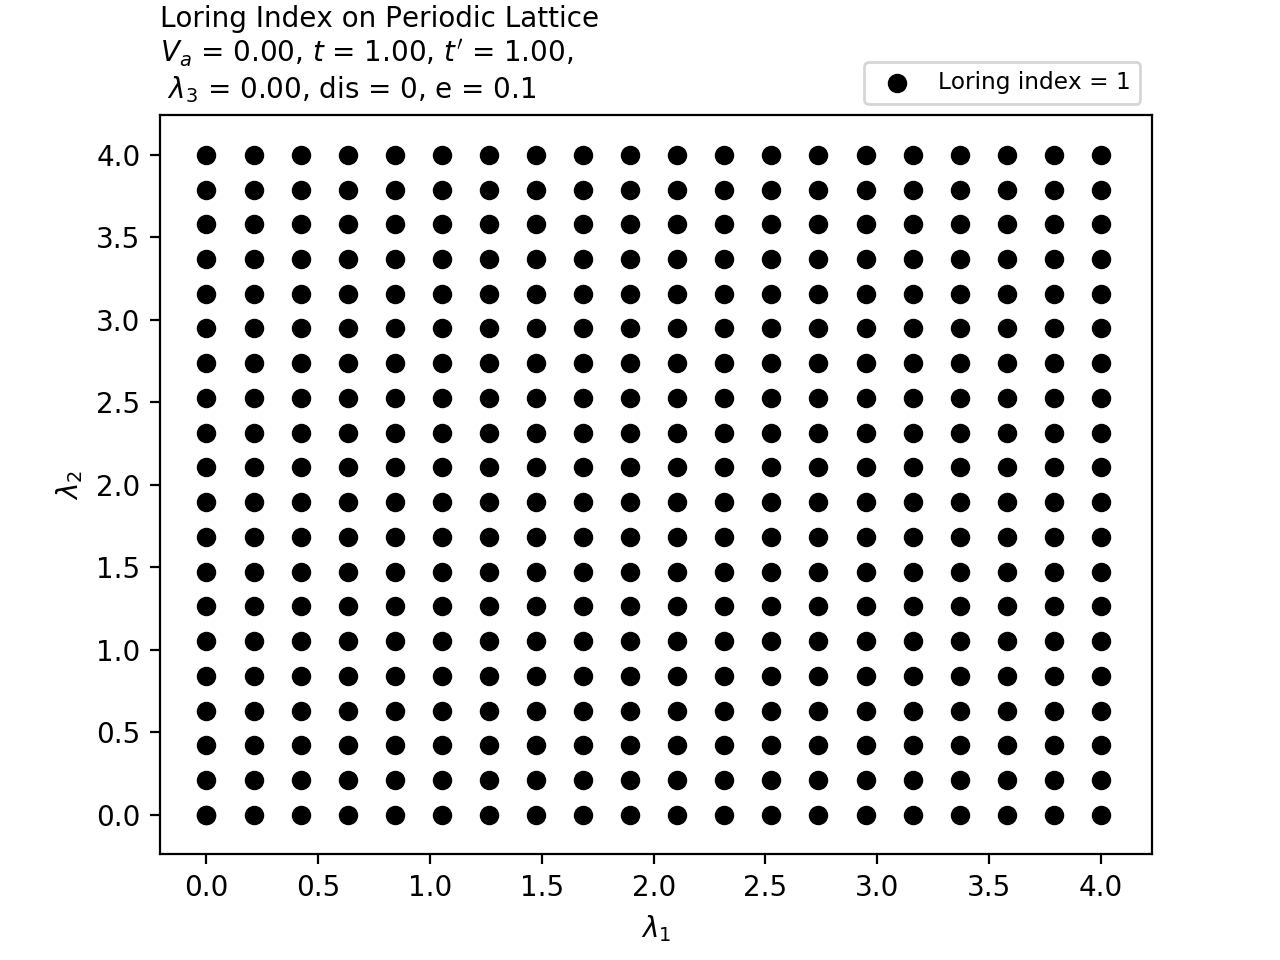
\includegraphics[width=.45\linewidth]{figures/periodic_top} }}%

\subfloat{{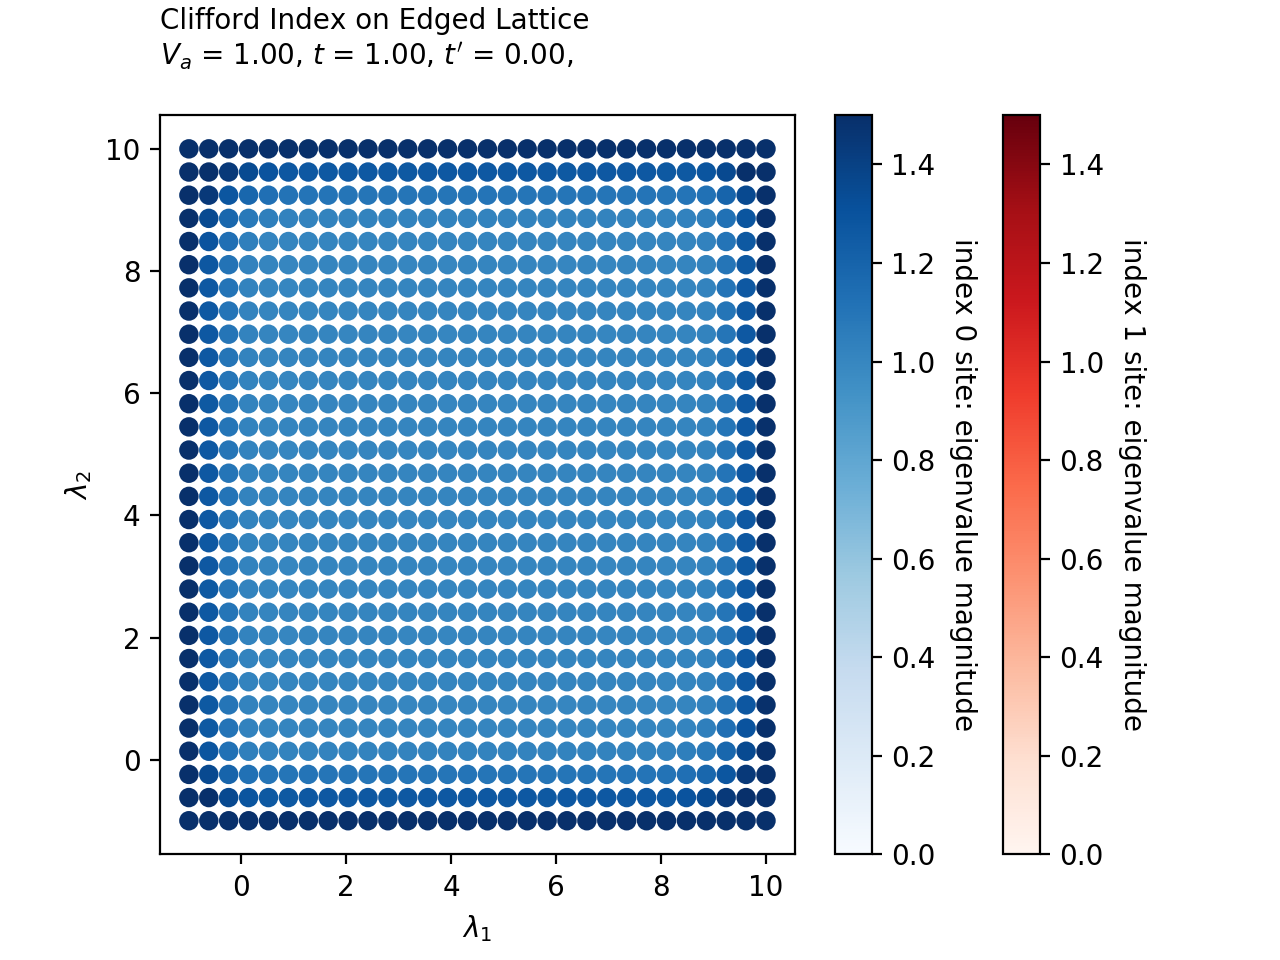
\includegraphics[width =.45\linewidth]{figures/edged_triv} }}%
\subfloat{{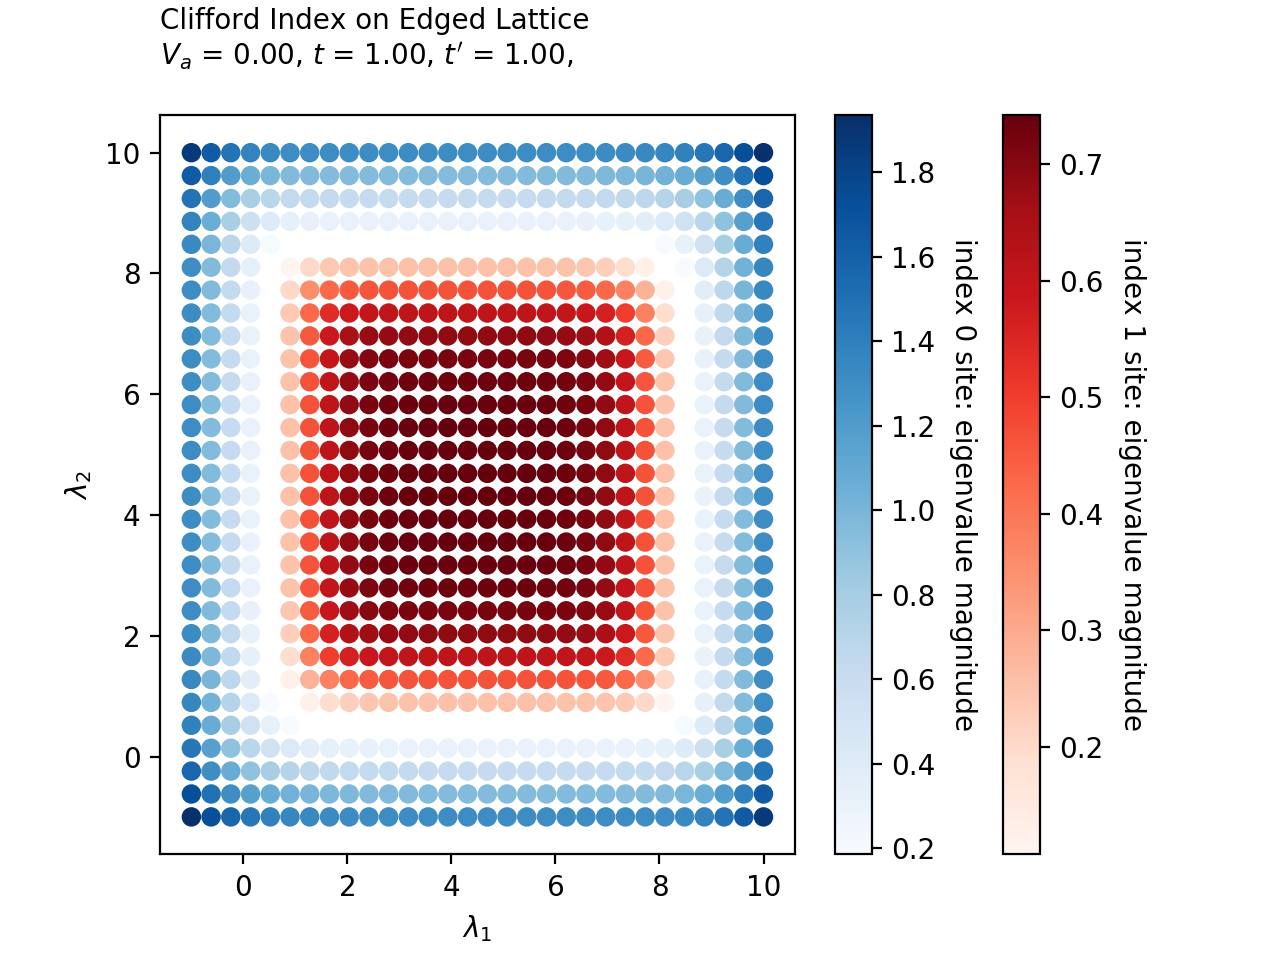
\includegraphics[width =.45\linewidth]{figures/edged_top} }}%
\caption{The top left is a trivial, periodic lattice; the top right is a topological, periodic lattice; the bottom left is a trivial, edged lattice; and the bottom right is a topological, edged lattice. Each site in these figures represents a $(\lambda_1,\lambda_2,\lambda_3)$ triple with $\lambda_3 = 0$. If a site is red, then it is in the pseudo-spectrum, i.e. $B(X - \lambda_1, Y - \lambda_2, H - \lambda_3)$ has a near-zero eigenvalue. If a site is not in the pseudo-spectrum, then it is colored black for Loring index 1 and white for Loring index 0, where the Loring index is defined as the signature of $B$.\\
}%
\label{fig:Loring Haldane}%
\end{figure}
The advantage of the Loring index compared to the Chern number is that the Chern number can only be defined on a periodic structure, whereas the Loring index can be computed on non-periodic media. We will use this advantage to study the robustness of waves on non-periodic media.

\section{Propagation in Haldane Model}

\aw{Clarify that this shows that the Bott index and Chern number predict edge states similarly}

As expected, we find that localized waves propagate along the boundary of the edged, topological lattice since this is a boundary between Loring index 0 and Loring index 1.

\section{\texorpdfstring{$p_x + ip_y$}{px + ipy} Model}
\aw{We should mention why we work with a different model: the point is that it is unclear how to generalize the Haldane model to disordered media.}
\section{Loring Index in \texorpdfstring{$p_x + ip_y$}{px + ipy} Model}
\section{Propagation in \texorpdfstring{$p_x + ip_y$}{px + ipy} Model}
\aw{This is a good ordering of things.}

\end{document}
